% Source: Corsin Nick/Class Notes/Week 11.pdf, pp. 2--15
\chapter{Week 11 --- Differential Forms}
\label{ch:week11}

% Transition: Claude Sonnet 5
This chapter closes the discussion of Gauss' theorem from Week 10 with two pieces of
intuition Corsin adds afterwards --- the case $n=1$, where the theorem degenerates to the
fundamental theorem of calculus, and a direct proof of the theorem for a square in
$\mathbb{R}^2$, built entirely from the FTC and Fubini --- and then turns to
\newterm{differential forms}: antisymmetric $k$-linear maps built to be reparametrization
invariant by construction, the wedge product that combines them, and the exterior derivative
$d$ that generalizes the gradient, curl, and divergence into a single operator. The exercise
sheet is at the end of the chapter, in \Cref{sec:week11_solutions}.

\section{Gauss' theorem revisited: the case \texorpdfstring{$n=1$}{n=1}, and a direct proof
for a square}
\label{sec:gauss_intuition}
\continuedfrom{sec:flux_divergence_theorem}

% Source: Corsin Nick/Class Notes/Week 11.pdf, p. 2
Gauss' theorem (\cref{thm:gauss_divergence}) is, in a precise sense, a higher-dimensional
fundamental theorem of calculus: it trades a derivative integrated over a region for the
original quantity evaluated on the region's boundary. Setting $n=1$ makes the analogy
literal. Let $f \in C^1([a,b])$, viewed as a (one-dimensional) vector field. Since $\divg f =
f'$ in dimension $1$, Gauss' formula becomes
\[\int_a^b \frac{\partial f}{\partial x}\,dx = \int_{[a,b]} \divg f\,d\vol_1
  = \int_{\partial[a,b]} \langle f,\nu\rangle\,d\vol_0
  = f(b) - f(a) \qquad \text{(FTC, almost).}\]
The last step identifies $\int_{\partial[a,b]} \langle f,\nu\rangle\,d\vol_0$ with $f(b)-f(a)$
by treating $\partial[a,b] = \{a,b\}$ as a $0$-dimensional submanifold with outward unit
normals $\nu(a) = -1$, $\nu(b) = +1$, and $\vol_0$ as counting measure.

\begin{ainote}
Corsin flags this himself: \qt{there are several problems with this argument, for example
what a $0$-dim Jordan measure or $0$-dim submanifold is}, and notes that \qt{the definitions
from the lecture can be extended to include this case} without carrying out the extension.
The word \qt{almost} above is his. Not pursued further here; the point of the calculation is
the analogy with the FTC, not a rigorous $n=1$ instance of \cref{thm:gauss_divergence}.
\end{ainote}

% Source: Corsin Nick/Class Notes/Week 11.pdf, p. 3
\begin{proof}[Proof of \cref{thm:gauss_divergence} for $n=2$, $B = (0,1)^2$]
Conversely, the fundamental theorem of calculus can be used to \emph{prove} Gauss' theorem;
we carry this out for the unit square. Let $F : [0,1]^2 \to \mathbb{R}^2$ be a $C^1$ vector
field and $B := (0,1)^2$. The boundary $\partial B$ splits into four edges, with outward unit
normals $-e_1$, $e_1$, $-e_2$, $e_2$ on the left, right, bottom, and top edges respectively.

% Sonnet 5 (Medium) --- FIG-W11-01
\begin{center}
\begin{tikzpicture}[>=Latex, scale=1.6]
  \draw[thick] (0,0) rectangle (1,1);
  \draw[->] (0,0.5) -- (-0.6,0.5) node[left, font=\scriptsize] {$-e_1$};
  \draw[->] (1,0.5) -- (1.6,0.5) node[right, font=\scriptsize] {$e_1$};
  \draw[->] (0.5,0) -- (0.5,-0.6) node[below, font=\scriptsize] {$-e_2$};
  \draw[->] (0.5,1) -- (0.5,1.6) node[above, font=\scriptsize] {$e_2$};
  \node[below left, font=\scriptsize] at (0,0) {$(0,0)$};
  \node[below right, font=\scriptsize] at (1,0) {$(1,0)$};
  \node[above left, font=\scriptsize] at (0,1) {$(0,1)$};
  \node[above right, font=\scriptsize] at (1,1) {$(1,1)$};
\end{tikzpicture}
\end{center}

Parametrizing each edge by $t \mapsto (0,t)$, $(1,t)$, $(t,0)$, $(t,1)$ for $t \in [0,1]$,
\[
\int_{\partial B} \langle F,\nu\rangle\,d\vol_1
  = \int_0^1 \langle F(0,t),-e_1\rangle\,dt + \int_0^1 \langle F(1,t),e_1\rangle\,dt
  + \int_0^1 \langle F(t,0),-e_2\rangle\,dt + \int_0^1 \langle F(t,1),e_2\rangle\,dt.
\]
Grouping the first pair and the second pair,
\[
\int_{\partial B} \langle F,\nu\rangle\,d\vol_1
  = \int_0^1 \big[F_1(1,t) - F_1(0,t)\big]\,dt + \int_0^1 \big[F_2(t,1) - F_2(t,0)\big]\,dt.
\]
By the fundamental theorem of calculus applied to $t \mapsto F_1(s,t)$ along $s$ and to
$s \mapsto F_2(t,s)$ along the second variable,
\[
\int_{\partial B} \langle F,\nu\rangle\,d\vol_1
  = \int_0^1\!\!\left(\int_0^1 \partial_1 F_1(s,t)\,ds\right) dt
  + \int_0^1\!\!\left(\int_0^1 \partial_2 F_2(t,s)\,ds\right) dt,
\]
and by Fubini,
\[
\int_{\partial B} \langle F,\nu\rangle\,d\vol_1
  = \int_B \partial_1 F_1\,d\vol_2 + \int_B \partial_2 F_2\,d\vol_2
  = \int_B \divg F\,d\vol_2. \qedhere
\]
\end{proof}

\section{Antisymmetric \texorpdfstring{$k$}{k}-linear forms and the wedge product}
\label{sec:antisymmetric_forms}

% Source: Corsin Nick/Class Notes/Week 11.pdf, p. 4
\begin{ainote}[Motivation]
Suppose one studies a submanifold $\mathcal{M} \subseteq \mathbb{R}^n$ via a parametrization
$\phi : D \to \mathcal{M}$, and integrates some quantity over $\mathcal{M}$ (for instance the
Gauss curvature, as in the Gauss--Bonnet theorem). The natural question is whether the
resulting number is a property of $\phi$, or a property of $\mathcal{M}$ itself: if it is
invariant under reparametrization, it must be the latter. \newterm{Differential forms} are
built to satisfy exactly this property. For a diffeomorphism $\Psi : V \to D$ with
$\det D\Psi > 0$ and a form $\omega$,
\begin{align}
\int_{\mathcal{M}} \omega &= \int_D \omega_{\phi(x)}(D\phi_x)\,dx \nonumber \\
  &\overset{\text{change of var.}}{=} \int_V \omega_{\phi(\Psi(y))}(D\phi_{\Psi(y)})
  \lvert\det D\Psi_y\rvert\,dy \nonumber \\
  &= \int_V \omega_{(\phi\circ\Psi)(y)}(D(\phi\circ\Psi)_y)\,dy = \int_{\mathcal{M}} \omega,
  \nonumber
\end{align}
where the middle equality uses the chain rule $D(\phi\circ\Psi)_y = D\phi_{\Psi(y)}\,D\Psi_y$
together with multilinearity and $\det D\Psi_y = \lvert\det D\Psi_y\rvert$. This calculation
is precisely why $\omega$ must be built from multilinear, antisymmetric maps: multilinearity
lets the Jacobian $D\Psi_y$ factor out as $\det D\Psi_y$, matching the $\lvert\det
D\Psi_y\rvert$ produced by the change-of-variables formula, exactly when $\det D\Psi_y > 0$.
\end{ainote}

% Source: Corsin Nick/Class Notes/Week 11.pdf, p. 5
\begin{definition}[Antisymmetric $k$-linear form]
\label{def:antisymmetric_k_linear_form}
Let $V$ be an $n$-dimensional real vector space and let $L : V^k \to \mathbb{R}$. Then $L$ is
an \newterm{antisymmetric $k$-linear form} (\germanterm{antisymmetrische $k$-lineare Form})
if
\begin{enumerate}[label=\textbf{(\alph*)}]
  \item \textbf{($k$-linear):} $L$ is linear in every entry:
  \[L(v_1,\ldots,\alpha v_i+\beta w_i,\ldots,v_k) = \alpha L(v_1,\ldots,v_i,\ldots,v_k)
    + \beta L(v_1,\ldots,w_i,\ldots,v_k);\]
  \item \textbf{(antisymmetric):} swapping any two entries negates the value:
  \[L(v_1,\ldots,v_i,\ldots,v_j,\ldots,v_k) = -L(v_1,\ldots,v_j,\ldots,v_i,\ldots,v_k).\]
\end{enumerate}
\end{definition}

\begin{remark}
For $k=n$ and $V = \mathbb{R}^n$, the normalization $L(e_1,\ldots,e_n) = 1$ pins down a
\emph{unique} such $L$, namely $L = \det$.
\end{remark}

\begin{notation}
For $v \in V$ and a fixed basis $(e_1,\ldots,e_n)$ of $V$, superscripts index the coordinates
of a single vector, $v = \sum_{i=1}^n v^i e_i = (v^1,\ldots,v^n)$, while subscripts index a
list of vectors $v_1,\ldots,v_k \in V$ --- this distinguishes \qt{the $i$-th coordinate of
$v$} from \qt{the $i$-th vector in the list}. From here on, $V = \mathbb{R}^n$ with the
standard basis.
\end{notation}

% Source: Corsin Nick/Class Notes/Week 11.pdf, p. 6
\begin{aiexample}[Two families of examples]
% Generator: Claude Sonnet 5 (Medium)
\begin{enumerate}[label=\textbf{\arabic*.}]
  \item Fix $A \in \mathrm{Mat}_{k\times n}(\mathbb{R})$. For $v_1,\ldots,v_k \in
  \mathbb{R}^n$, write $V := (v_1\mid\cdots\mid v_k) \in \mathrm{Mat}_{n\times k}(\mathbb{R})$
  for the matrix with these columns; then $AV \in \mathrm{Mat}_{k\times k}(\mathbb{R})$, and
  $L(v_1,\ldots,v_k) := \det(AV)$ is an antisymmetric $k$-linear form, since $\det$ is
  multilinear and antisymmetric in the columns of its argument, and $v \mapsto Av$ is linear.
  \item For $k=1$, $L : \mathbb{R}^n \to \mathbb{R}$ is a \newterm{covector},
  $L \in (\mathbb{R}^n)^*$. The standard basis $(e_1^*,\ldots,e_n^*)$ of $(\mathbb{R}^n)^*$,
  satisfying $e_i^*(e_j) = \delta_{ij}$, consists of $1$-forms; in particular
  $e_i^*(v) = v^i$.
\end{enumerate}
\end{aiexample}

\begin{remark}[An equivalent characterization]
In the lecture, antisymmetry was replaced by the equivalent condition
\[L(VA) = L(V)\det(A), \qquad V := (v_1,\ldots,v_k) \in \mathrm{Mat}_{n\times k}(\mathbb{R}),
  \quad A \in \mathrm{Mat}_{k\times k}(\mathbb{R}),\]
writing $L(V)$ for $L(v_1,\ldots,v_k)$. We verify the equivalence in the special case $n=3$,
$k=2$: let $V = (v\mid w) \in \mathrm{Mat}_{3\times2}(\mathbb{R})$ and $A = \begin{pmatrix} a &
b \\ c & d \end{pmatrix}$, so that $VA = (av+cw \mid bv+dw)$. Rewriting $L(VA)$ in bilinear
form and using $L(v,v) = -L(v,v) = 0$ (from antisymmetry) together with $L(w,v) = -L(v,w)$,
\begin{align}
L(VA) &= L(av+cw,\,bv+dw) \nonumber \\
  &= ab\,L(v,v) + ad\,L(v,w) + cb\,L(w,v) + cd\,L(w,w) \nonumber \\
  &= (ad-bc)\,L(v,w) = L(V)\det(A). \nonumber
\end{align}
\end{remark}

% Source: Corsin Nick/Class Notes/Week 11.pdf, p. 7
\begin{definition}[Wedge product]
\label{def:wedge_product}
For a $k$-form $\alpha$ and an $m$-form $\beta$ on $\mathbb{R}^n$, the \newterm{wedge product}
(\germanterm{Dachprodukt}) $\alpha \wedge \beta$ is the $(k+m)$-form
\[
(\alpha\wedge\beta)(v_1,\ldots,v_k,v_{k+1},\ldots,v_{k+m})
  = \sum_{\sigma \in S_{k,m}} \sgn(\sigma)\,\alpha(v_{\sigma(1)},\ldots,v_{\sigma(k)})\,
    \beta(v_{\sigma(k+1)},\ldots,v_{\sigma(k+m)}),
\]
where $S_{k,m}$ is the set of permutations $\sigma$ of $\{1,\ldots,k+m\}$ satisfying
$\sigma(1) < \cdots < \sigma(k)$ and $\sigma(k+1) < \cdots < \sigma(k+m)$ (the
\newterm{$(k,m)$-shuffles}).
\end{definition}

\begin{ainote}
Corsin calls this formula \qt{not terribly important for our purposes} and instead has us work
directly with the five properties below.
\end{ainote}

The following properties of $\wedge$ are the ones actually used:
\begin{enumerate}[label=\textbf{(\arabic*)}]
  \item $\wedge$ is bilinear.
  \item For $\alpha$ a $k$-form and $\beta$ an $m$-form, $\alpha\wedge\beta$ is a $(k+m)$-form.
  \item $(\alpha\wedge\beta)\wedge\gamma = \alpha\wedge(\beta\wedge\gamma) = \alpha\wedge\beta
  \wedge\gamma$ (associativity).
  \item For $1$-forms $L_1,\ldots,L_k$ and vectors $v_1,\ldots,v_k \in \mathbb{R}^n$,
  \[L_1\wedge L_2\wedge\cdots\wedge L_k(v_1,\ldots,v_k) = \det\big(L_i(v_j)\big)_{1\leq i,j
  \leq k}.\]
  \item For $\alpha(T) := \det(AT)$, $\beta(S) := \det(BS)$ as in \cref{def:antisymmetric_k_linear_form}
  example 1,
  \[\alpha\wedge\beta(X) = \det\!\left(\begin{bmatrix} A \\ B \end{bmatrix} X\right).\]
\end{enumerate}

% Source: Corsin Nick/Class Notes/Week 11.pdf, p. 8
\begin{example}
By property (4), for $1 \leq i_1 < \cdots < i_k \leq n$,
\[
e_{i_1}^*\wedge\cdots\wedge e_{i_k}^*(v_1,\ldots,v_k) = \det\!\left(
  \begin{pmatrix} v_1^{i_1} & \cdots & v_k^{i_1} \\ \vdots & \ddots & \vdots \\ v_1^{i_k} &
  \cdots & v_k^{i_k} \end{pmatrix}\right)
  = \det\!\left(\begin{bmatrix} e_{i_1}\transp \\ \vdots \\ e_{i_k}\transp \end{bmatrix}
  \begin{bmatrix} v_1 & \cdots & v_k \end{bmatrix}\right).
\]
\end{example}

% Source: Corsin Nick/Class Notes/Week 11.pdf, pp. 9--10
\begin{proposition}[Every $k$-linear form is a combination of wedge products of covectors]
\label{prop:k_form_basis_expansion}
Every antisymmetric $k$-linear form $L$ on $\mathbb{R}^n$ can be written as
\[L = \sum_{1\leq i_1<\cdots<i_k\leq n} \ell_{i_1\cdots i_k}\,e_{i_1}^*\wedge\cdots\wedge
  e_{i_k}^*\]
for uniquely determined scalars $\ell_{i_1\cdots i_k} \in \mathbb{R}$.
\end{proposition}

\begin{proof}
Expand each argument $v_i = \sum_{m=1}^n v_i^m e_m$ and use $k$-linearity:
\[L(v_1,\ldots,v_k) = L\!\left(\sum_{i_1=1}^n v_1^{i_1}e_{i_1},\ldots,\sum_{i_k=1}^n
  v_k^{i_k}e_{i_k}\right) = \sum_{1\leq i_1,\ldots,i_k\leq n} L(e_{i_1},\ldots,e_{i_k})\,
  v_1^{i_1}\cdots v_k^{i_k}.\]
By antisymmetry, $L(e_{i_1},\ldots,e_{i_k}) = 0$ whenever two indices coincide, so the sum may
be restricted to $i_1,\ldots,i_k$ pairwise distinct; regrouping each such tuple by the
permutation $\sigma$ that sorts it into increasing order $i_{\sigma(1)}<\cdots<i_{\sigma(k)}$,
\begin{align}
L(v_1,\ldots,v_k) &= \sum_{1\leq i_1<\cdots<i_k\leq n} L(e_{i_1},\ldots,e_{i_k})
  \sum_{\sigma\in S_k} \sgn(\sigma)\,v_1^{i_{\sigma(1)}}\cdots v_k^{i_{\sigma(k)}} \nonumber \\
  &= \sum_{1\leq i_1<\cdots<i_k\leq n} \ell_{i_1\cdots i_k}\,e_{i_1}^*\wedge\cdots\wedge
  e_{i_k}^*(v_1,\ldots,v_k), \nonumber
\end{align}
with $\ell_{i_1\cdots i_k} := L(e_{i_1},\ldots,e_{i_k})$, using that the inner sum over $\sigma$
is exactly the determinant expansion of $e_{i_1}^*\wedge\cdots\wedge e_{i_k}^*(v_1,\ldots,v_k)$
from property (4) above.
\end{proof}

\section{Differential forms and the exterior derivative}
\label{sec:differential_forms}

% Source: Corsin Nick/Class Notes/Week 11.pdf, p. 10
\begin{definition}[Differential form]
\label{def:differential_p_form}
A \newterm{differential $p$-form} $\omega$ (\germanterm{Differentialform}) is defined on a
domain $D \subseteq \mathbb{R}^n$ if, for every $x \in D$, $\omega(x) = \omega_x : (\mathbb{R}^n)^p
\to \mathbb{R}$ is an antisymmetric $p$-linear map. Since $(e_1(x),\ldots,e_n(x))$ is a basis
of $\mathbb{R}^n$ for every $x \in D$, \cref{prop:k_form_basis_expansion} lets us write
\[\omega(x) = \sum_{1\leq i_1<\cdots<i_p\leq n} \omega_{i_1\cdots i_p}(x)\,e_{i_1}^*(x)\wedge
  \cdots\wedge e_{i_p}^*(x)\]
for functions $\omega_{i_1\cdots i_p} : \mathbb{R}^n \to \mathbb{R}$.
\end{definition}

% Source: Corsin Nick/Class Notes/Week 11.pdf, p. 11
\begin{notation}
We abbreviate $e_{i_1}^*\wedge\cdots\wedge e_{i_p}^* =: e_I^*$ for $I = (i_1,\ldots,i_p)$, and
write $\Omega^p(U)$ for the set of $p$-forms on $U \subseteq \mathbb{R}^n$. By convention,
$\Omega^0(U) = C^\infty(U)$.
\end{notation}

\begin{example}
Let $U \subseteq \mathbb{R}^n$.
\begin{enumerate}[label=\textbf{\arabic*.}]
  \item Any $f \in C^\infty(U)$ is a $0$-form.
  \item A vector field $F : U \to \mathbb{R}^n$ has an associated $1$-form $\omega_F(x) : v
  \mapsto \langle F(x),v\rangle$, that is,
  \[\omega_F(x)(v) = \sum_{i=1}^n F^i(x)\,v^i = \sum_{i=1}^n F^i(x)\,e_i^*(x)(v)
    \qquad\Longrightarrow\qquad \omega_F = \sum_{i=1}^n F^i\,e_i^*.\]
% Source: Corsin Nick/Class Notes/Week 11.pdf, p. 12
  \item $F : U \to \mathbb{R}^n$ also naturally induces an $(n-1)$-form
  \[\omega_F^{n-1}(x)(v_1,\ldots,v_{n-1}) := \det\big(F(x)\mid v_1\mid\cdots\mid v_{n-1}\big).\]
  Developing this determinant along the first column,
  \begin{align}
  \omega_F^{n-1}(x)(v_1,\ldots,v_{n-1}) &= \sum_{i=1}^n (-1)^{i-1}F^i(x)\det\!\left(
    \begin{smallmatrix} v_1^1 & \cdots & v_{n-1}^1 \\ \vdots & & \vdots \\ v_1^{i-1} & \cdots &
    v_{n-1}^{i-1} \\ v_1^{i+1} & \cdots & v_{n-1}^{i+1} \\ \vdots & & \vdots \\ v_1^n &
    \cdots & v_{n-1}^n \end{smallmatrix}\right) \nonumber \\
    &= \sum_{i=1}^n (-1)^{i-1}F^i(x)\,e_1^*\wedge\cdots\wedge\widehat{e_i^*}\wedge\cdots\wedge
    e_n^*(v_1,\ldots,v_{n-1}), \nonumber
  \end{align}
  where $\widehat{e_i^*}$ denotes an omitted factor, so that $\omega_F^{n-1} =
  \sum_{i=1}^n (-1)^{i-1}F^i\,e_1^*\wedge\cdots\wedge\widehat{e_i^*}\wedge\cdots\wedge e_n^*$.
  \item In particular, for $F : \mathbb{R}^3 \to \mathbb{R}^3$,
  \[\omega_F^2(x)(v_1,v_2) = \langle F(x),v_1\times v_2\rangle = \det\big(F(x)\mid v_1\mid
    v_2\big).\]
\end{enumerate}
\end{example}

\begin{ainote}
Item 4 identifies $\omega_F^2$ with the flux integrand from \cref{sec:flux_divergence_theorem}
in Week 10: the flux $\int_S \langle F,\nu\rangle\,d\vol_2$ over a parametrized surface is
exactly the integral, in the sense of the motivating change-of-variables calculation above, of
the $2$-form $\omega_F^2$.
\end{ainote}

% Source: Corsin Nick/Class Notes/Week 11.pdf, p. 13
\begin{theorem}[Exterior derivative]
\label{thm:exterior_derivative}
There exists a unique linear operator $d : \Omega^k(U) \to \Omega^{k+1}(U)$ satisfying
\begin{enumerate}[label=\textbf{(\arabic*)}]
  \item for $f \in C^\infty(U) = \Omega^0(U)$: $df = Df$, the ordinary differential;
  \item for $\omega \in \Omega^k(U)$, $\theta \in \Omega^s(U)$: $d(\omega\wedge\theta) =
  d\omega\wedge\theta + (-1)^k\,\omega\wedge d\theta$;
  \item $d\circ d\,\omega = d^2\omega = 0$.
\end{enumerate}
\end{theorem}

\begin{ainote}
Corsin states this as a fact seen in the lecture, without proof, and moves directly to its
consequences. Not reproduced here for the same reason.
\end{ainote}

Denote by $dx^i$ the differential of $x \mapsto x^i$ in a moving frame $(e_1(x),\ldots,e_n(x))$,
that is, $dx^i = e_i^*(x)$. Every $p$-form $\omega$ on $U \subseteq \mathbb{R}^n$ then takes
the shape
\[\omega = \sum_{1\leq i_1<\cdots<i_p\leq n} \omega_{i_1\cdots i_p}\,dx^{i_1}\wedge\cdots\wedge
  dx^{i_p} = \sum_I \omega_I\,dx^I, \qquad \omega_I \in C^\infty(U),\]
with exterior derivative
\[d\omega = \sum_I d\omega_I \wedge dx^I.\]

% Source: Corsin Nick/Class Notes/Week 11.pdf, pp. 14--15
\begin{example}[The exterior derivative recovers the gradient and the curl]
\label{ex:exterior_derivative_gradient_curl}
\begin{enumerate}[label=\textbf{\arabic*.}]
  \item For $f \in C^\infty(\mathbb{R}^n) = \Omega^0(\mathbb{R}^n)$,
  \[df_x(v) = \left(\frac{\partial f}{\partial x^1}\ \Big|\ \cdots\ \Big|\ \frac{\partial f}
    {\partial x^n}\right)\!\begin{pmatrix}v^1\\ \vdots \\ v^n\end{pmatrix}
    = \frac{\partial f}{\partial x^1}\,dx^1(v) + \cdots + \frac{\partial f}{\partial x^n}\,
    dx^n(v),\]
  so $df = \frac{\partial f}{\partial x^1}\,dx^1 + \cdots + \frac{\partial f}{\partial x^n}\,
  dx^n = \langle \nabla f,\cdot\rangle$: the exterior derivative of a $0$-form is exactly the
  $1$-form associated (as in the example above) to the gradient vector field $\nabla f$. This
  is the shape that makes Stokes' theorem specialize to the FTC, as in
  \cref{sec:gauss_intuition}.
  \item Define a $1$-form on $U \subseteq \mathbb{R}^3$ by $\omega(x,y,z) = \langle
  F(x,y,z),\cdot\rangle = F^1\,dx+F^2\,dy+F^3\,dz$ for a vector field $F$. By property (2) of
  \cref{thm:exterior_derivative} and $d(dx^i)=0$ (since $dx^i = d(x^i)$ and $d^2=0$),
  \[
  d\omega = dF^1\wedge dx + dF^2\wedge dy + dF^3\wedge dz,
  \]
  and expanding each $dF^i = \partial_x F^i\,dx+\partial_y F^i\,dy+\partial_z F^i\,dz$, only
  the cross terms survive the wedge (since $dx^i\wedge dx^i=0$ by antisymmetry):
  \[
  d\omega = \Big(\frac{\partial F^3}{\partial y}-\frac{\partial F^2}{\partial z}\Big)dy\wedge
    dz + \Big(\frac{\partial F^1}{\partial z}-\frac{\partial F^3}{\partial x}\Big)dz\wedge dx
    + \Big(\frac{\partial F^2}{\partial x}-\frac{\partial F^1}{\partial y}\Big)dx\wedge dy.
  \]
  Comparing with example item 4 in \cref{sec:differential_forms}, this is exactly
  $\omega_{\nabla\times F}^2 = \langle\nabla\times F,\cdot\times\cdot\rangle = \det(\nabla
  \times F\mid\cdot\mid\cdot)$: the exterior derivative of the $1$-form associated to $F$ is
  the $2$-form associated to $\curl F$.
  \end{enumerate}
\end{example}

\begin{ainote}
Corsin leaves the middle expansion of $d\omega$ --- nine terms, one for each pair
$(dF^i,dx^j)$ --- fully written out before collecting the six that survive into the three
coefficient pairs above; condensed here to the surviving terms directly, since $dx\wedge
dx=dy\wedge dy=dz\wedge dz=0$ kills exactly the three diagonal terms and antisymmetry
($dy\wedge dx=-dx\wedge dy$, etc.) pairs up the rest.
\end{ainote}

% Supplement: Sascha Brack/Class Notes/Week_11_Notes_Friday.pdf, pp. 2--4
\subsection{Sneak peek at Stokes' theorem}
\label{sec:stokes_sneak_peek}

\begin{ainote}
Before the formal introduction of Stokes' theorem in Week 12, Sascha presented introductory examples to build intuition. The classical version of Stokes' theorem states that for a surface $A \subset \mathbb{R}^3$ and a vector field $F$,
\[\int_A (\curl F)\cdot \nu \mathop{d\text{vol}}_2 = \int_{\partial A} F \cdot \tau \,dL,\]
where $\nu$ is the unit normal to $A$ and $\tau$ is the unit tangent vector to the boundary curve $\partial A$.
\end{ainote}

\begin{example}[Stokes' theorem on a hemisphere]
\label{ex:stokes_hemisphere}
Let $A := \{(x,y,z) \in \mathbb{R}^3 \mid x^2+y^2+z^2=1,\ z \geq 0\}$ be the upper hemisphere.
Given the vector field $F(x,y,z) := (z^2, x^2, y^2)\transp$, we can evaluate both sides of Stokes' theorem.
\begin{enumerate}[label=\textbf{\arabic*.}]
    \item \textbf{The rotation of $F$:} $\curl F = \nabla \times F = (2y, 2z, 2x)\transp$.
    \item \textbf{The surface normal:} On the unit sphere, the outward normal is simply $\nu(x,y,z) = (x,y,z)\transp$.
    \item \textbf{The boundary $\partial A$:} The boundary of the upper hemisphere is the unit circle in the $xy$-plane, $x^2+y^2=1$ with $z=0$. This can be parametrized by the closed path $\gamma : [0,2\pi] \to \mathbb{R}^3$,
    \[\gamma(t) = \begin{pmatrix} \cos t \\ \sin t \\ 0 \end{pmatrix}.\]
\end{enumerate}
Evaluating the path integral (the right-hand side of Stokes' theorem):
\[\int_{\partial A} F \cdot \tau \,dL = \int_0^{2\pi} F(\gamma(t)) \cdot \gamma'(t) \,dt.\]
Since $z=0$ on $\gamma$, we have $F(\gamma(t)) = (0, \cos^2 t, \sin^2 t)\transp$. The derivative is $\gamma'(t) = (-\sin t, \cos t, 0)\transp$.
\[\int_0^{2\pi} \begin{pmatrix} 0 \\ \cos^2 t \\ \sin^2 t \end{pmatrix} \cdot \begin{pmatrix} -\sin t \\ \cos t \\ 0 \end{pmatrix} dt = \int_0^{2\pi} \cos^3 t \,dt = 0.\]
\end{example}

\begin{example}[Path integral using Stokes' theorem]
\label{ex:stokes_path_integral}
Compute $\oint_\Gamma F \cdot \tau \,dL$ where $F(x,y,z) := (x, y, z)\transp$ and $\Gamma$ is the unit circle in the $xy$-plane (oriented counter-clockwise).

Instead of computing the line integral directly, we can use Stokes' theorem. The curve $\Gamma$ bounds the unit disk $A = \{(x,y,0) \mid x^2+y^2 \leq 1\}$.
First, we compute the rotation of $F$:
\[\curl F = \nabla \times F = \begin{pmatrix} \partial_y(z) - \partial_z(y) \\ \partial_z(x) - \partial_x(z) \\ \partial_x(y) - \partial_y(x) \end{pmatrix} = \begin{pmatrix} 0 \\ 0 \\ 0 \end{pmatrix}.\]
By Stokes' theorem, the line integral along $\Gamma$ bounds a surface $A$ on the sphere (for example, the upper hemisphere). The surface integral is:
\[\oint_\Gamma F \cdot \tau \,dL = \int_A (\curl F) \cdot \nu \mathop{d\text{vol}}_2 = 0.\]
\end{example}

% Supplement: Sascha Brack/Class Notes/Week_11_Notes_Monday.pdf, pp. 5--10
\subsection{Green's theorem and conservative fields}
\label{sec:greens_theorem_conservative_fields}

\begin{ainote}
Green's theorem, conservative vector fields, and path integrals were also discussed in the Monday session. 
\end{ainote}

\begin{theorem}[Green's Theorem]
\label{thm:greens_theorem}
Let $F : U \to \mathbb{R}^2$ be a continuously differentiable vector field on an open set $U \subseteq \mathbb{R}^2$. Then, for any compact $C^1$ domain $\Omega \subseteq U$,
\[\int_\Omega \curl F \mathop{d\text{vol}}_2 = \int_{\partial\Omega} F \cdot \tau \,dL,\]
where $\tau$ is the unit tangent vector to the boundary $\partial\Omega$ oriented counter-clockwise (i.e.\ $\tau = (-\nu_2, \nu_1)\transp$, with $\nu$ being the outward unit normal).
\end{theorem}

\begin{ainote}
% Supplement: Sascha Brack/Class Notes/Week_10_Notes_Monday.pdf, p. 16
\begin{center}
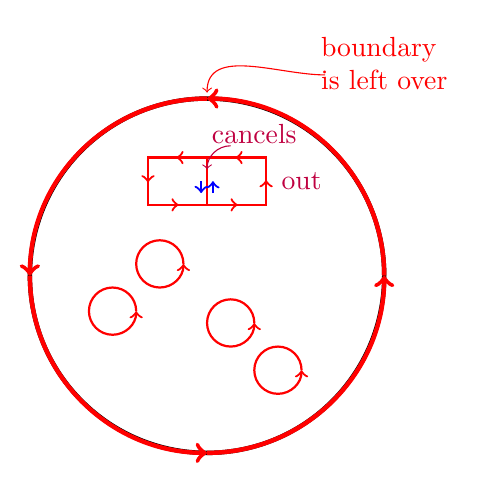
\begin{tikzpicture}[scale=1.5]
  % Domain
  \draw[ultra thick] (0,0) circle (1.5);
  % Boundary orientation
  \draw[red, ultra thick, ->] (1.5,0) arc (0:90:1.5);
  \draw[red, ultra thick, ->] (0,1.5) arc (90:180:1.5);
  \draw[red, ultra thick, ->] (-1.5,0) arc (180:270:1.5);
  \draw[red, ultra thick, ->] (0,-1.5) arc (270:360:1.5);
  
  \node[red, align=left] at (1.5, 1.8) {boundary\\is left over};
  \draw[red, ->] (1.0, 1.7) to[out=180, in=90] (0, 1.55);
  
  % Internal rotations
  \foreach \x/\y in {-0.6/-0.3, 0.4/-0.4, -0.2/0.1, 0.8/-0.8} {
    \draw[red, thick, ->] (\x,\y) arc (0:360:0.2);
  }
  
  % Two cancelling squares
  \draw[red, thick] (-0.5, 0.6) rectangle (0, 1.0);
  \draw[red, thick] (0, 0.6) rectangle (0.5, 1.0);
  % arrows
  \draw[red, thick, ->] (-0.25, 1.0) -- (-0.26, 1.0);
  \draw[red, thick, ->] (0.25, 1.0) -- (0.24, 1.0);
  \draw[red, thick, ->] (-0.5, 0.8) -- (-0.5, 0.79);
  \draw[red, thick, ->] (0.5, 0.8) -- (0.5, 0.81);
  \draw[red, thick, ->] (-0.25, 0.6) -- (-0.24, 0.6);
  \draw[red, thick, ->] (0.25, 0.6) -- (0.26, 0.6);
  
  \draw[blue, thick, ->] (-0.05, 0.8) -- (-0.05, 0.7);
  \draw[blue, thick, ->] (0.05, 0.7) -- (0.05, 0.8);
  
  \node[purple] at (0.4, 1.2) {cancels};
  \node[purple] at (0.8, 0.8) {out};
  \draw[purple, ->] (0.2, 1.1) to[out=180, in=90] (0, 0.9);
  
\end{tikzpicture}
\end{center}
We integrate the rotation inside the domain. Basically all the \qt{intermediate values} cancel out because for two points close to each other, the rotation points in opposite directions. Only the boundary is left over in the end!
\end{ainote}

\begin{example}[Area of a region via Green's theorem]
\label{ex:area_greens_theorem}
Consider a region $\Omega \subseteq \mathbb{R}^2$ defined by the region inside the curve $x^{2/3} + y^{2/3} = 1$ in the first quadrant, bounded by the axes. The curve can be parametrized as $\varphi(t) = (\cos^3 t, \sin^3 t)\transp$ for $t \in [0, \pi/2]$.

The area is $\vol_2(\Omega) = \int_\Omega 1 \mathop{d\text{vol}}_2$. We look for a vector field $F$ such that $\curl F = \partial_x F_2 - \partial_y F_1 \equiv 1$ on $\Omega$. A simple choice is $F(x,y) := (0, x)\transp$.
By Green's theorem, we have:
\[\vol_2(\Omega) = \int_\Omega \curl F \mathop{d\text{vol}}_2 = \int_{\partial\Omega} F \cdot \tau \,dL = \int_0^{\pi/2} F(\varphi(t)) \cdot \varphi'(t) \,dt.\]
Since $\tau(\varphi(t)) \,dL = \varphi'(t) \,dt$ along the parametrization, we compute the dot product:
\[F(\varphi(t)) \cdot \varphi'(t) = \begin{pmatrix} 0 \\ \varphi_1(t) \end{pmatrix} \cdot \begin{pmatrix} \varphi_1'(t) \\ \varphi_2'(t) \end{pmatrix} = \varphi_1(t)\varphi_2'(t).\]
This turns the area computation into a single 1D integral in $t$.
\end{example}

\begin{definition}[Conservative vector field]
\label{def:conservative_field}
Given a $C^k$ vector field $F$ on an open set $U \subseteq \mathbb{R}^n$, we call it \newterm{conservative} if there exists a scalar field $f : U \to \mathbb{R}$ of class $C^{k+1}$ such that $F \equiv \nabla f$. The function $f$ is called a \newterm{potential} for $F$.
\end{definition}

\begin{lemma}[Integrability conditions]
\label{lem:integrability_conditions}
Let $U \subseteq \mathbb{R}^n$ be open, and let $F$ be a $C^1$ conservative vector field on $U$ with components $F_1, \dots, F_n$. Then we necessarily have the integrability conditions:
\[\partial_j F_k = \partial_k F_j \qquad \text{for all } j, k \in \{1,\dots,n\}.\]
\end{lemma}
\begin{proof}
Let $f$ be a potential such that $F = \nabla f = (\partial_1 f, \dots, \partial_n f)\transp$. Then by Schwarz's theorem (symmetry of second derivatives),
\[\partial_j F_k = \partial_j(\partial_k f) = \partial_j\partial_k f = \partial_k\partial_j f = \partial_k(\partial_j f) = \partial_k F_j.\qedhere\]
\end{proof}

\begin{proposition}[Work along a path as difference of potential]
\label{prop:work_difference_potential}
Let $U \subseteq \mathbb{R}^n$ be open, and let $F : U \to \mathbb{R}^n$ be a continuous conservative vector field with potential $f$. Then for any $C^1$ path $\gamma : [0,1] \to U$, the line integral of $F$ along $\gamma$ depends only on the endpoints:
\[\int_\gamma F \cdot d\gamma = f(\gamma(1)) - f(\gamma(0)).\]
\end{proposition}
\begin{proof}
By definition of the path integral and the chain rule,
\begin{align*}
\int_\gamma F \cdot d\gamma &= \int_0^1 F(\gamma(t)) \cdot \gamma'(t) \,dt = \int_0^1 \nabla f(\gamma(t)) \cdot \gamma'(t) \,dt \\
&= \int_0^1 Jf(\gamma(t)) J\gamma(t) \,dt = \int_0^1 J(f \circ \gamma)(t) \,dt = \int_0^1 (f \circ \gamma)'(t) \,dt.
\end{align*}
By the fundamental theorem of calculus, this equals $(f \circ \gamma)(1) - (f \circ \gamma)(0) = f(\gamma(1)) - f(\gamma(0))$.
\end{proof}

\begin{example}[Line integral of a conservative field]
\label{ex:conservative_field_integral}
Consider the vector field $F : [0,1] \times [0,2] \to \mathbb{R}^2$ given by $F(x,y) := (y^2, 2xy)\transp$.
First, we show that $F$ is conservative by finding a potential $f$ such that $\nabla f = F$. We need $\partial_x f = y^2$ and $\partial_y f = 2xy$. Integrating the first equation with respect to $x$ gives $f(x,y) = xy^2 + c(y)$. Differentiating with respect to $y$ gives $\partial_y f = 2xy + c'(y)$, which must equal $2xy$. Thus $c'(y) = 0$, and we can choose $c(y) = 0$. The potential is $f(x,y) = xy^2$.

Now, let $\Gamma$ be a closed path on the boundary $\partial U$ of the domain, starting and ending at $\gamma(0) = \gamma(1) = (0,0)\transp$. By \cref{prop:work_difference_potential}, the line integral around this closed loop is simply the difference in potential at the endpoints:
\[\oint_\Gamma F \cdot d\gamma = f(\gamma(1)) - f(\gamma(0)) = f(0,0) - f(0,0) = 0.\]
\end{example}

\subsection{The Poincaré lemma and simply connected domains}
\label{sec:poincare_lemma_simply_connected}

\begin{theorem}[Poincaré Lemma]
\label{thm:poincare_lemma}
Let $U \subseteq \mathbb{R}^n$ be open, and let $\alpha \in \Omega^1(U)$ be a $C^1$ closed $1$-form, that is, $d\alpha = 0$.
Let $\gamma_0, \gamma_1 : [0,1] \to U$ be piecewise $C^1$ paths with the same initial point $x_0$ and the same endpoint $x_1$. Suppose that $\gamma_0$ and $\gamma_1$ are \newterm{homotopic} in $U$ with fixed endpoints. For simplicity, assume that the homotopy $H : [0,1]^2 \to U$ is smooth. Then
\[\int_{\gamma_0} \alpha = \int_{\gamma_1} \alpha.\]
\end{theorem}

\begin{corollary}[Existence of potentials in simply connected domains]
\label{cor:potentials_simply_connected}
Let $U \subseteq \mathbb{R}^n$ be an open \newterm{simply connected} set. Then every closed $C^1$ $1$-form on $U$ is exact. That is, if $\alpha \in \Omega^1(U)$ satisfies $d\alpha = 0$, then there exists a function $f \in C^2(U)$ such that $\alpha = df$.
Equivalently, if $F \in C^1(U, \mathbb{R}^n)$ satisfies the integrability conditions
\[\partial_j F_k = \partial_k F_j \qquad \text{for all } j, k \in \{1,\dots,n\},\]
then $F$ is conservative: there exists a potential $f \in C^2(U)$ such that $\nabla f = F$.
\end{corollary}

\begin{ainote}[Intuition on simply connected spaces]
A space $U$ is simply connected if any closed loop in $U$ can be continuously contracted to a point within $U$ (i.e.\ any two paths with the same endpoints are homotopic). 

% Supplement: Sascha Brack/Class Notes/Week_12_Notes_Monday.pdf, p. 7
\begin{center}
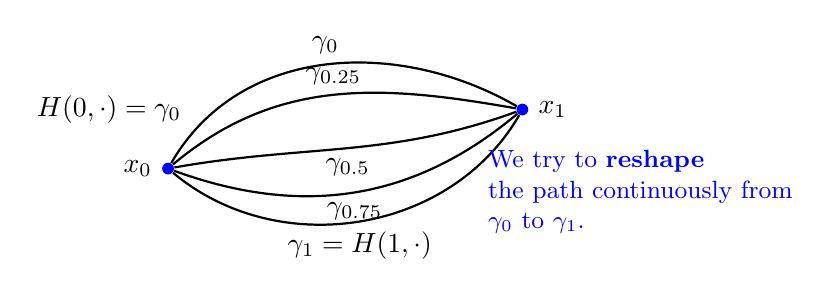
\begin{tikzpicture}[scale=1.5]
  \node[circle, fill=blue, inner sep=1.5pt, label=left:{$x_0$}] (x0) at (0,0) {};
  \node[circle, fill=blue, inner sep=1.5pt, label=right:{$x_1$}] (x1) at (3,0.5) {};
  
  \draw[thick] (x0) to[out=60, in=150] node[pos=0.5, above] {$\gamma_0$} (x1);
  \draw[thick] (x0) to[out=40, in=170] node[pos=0.5, above] {$\gamma_{0.25}$} (x1);
  \draw[thick] (x0) to[out=10, in=200] node[pos=0.5, below] {$\gamma_{0.5}$} (x1);
  \draw[thick] (x0) to[out=-20, in=220] node[pos=0.5, below] {$\gamma_{0.75}$} (x1);
  \draw[thick] (x0) to[out=-40, in=240] node[pos=0.5, below] {$\gamma_1 = H(1,\cdot)$} (x1);
  \node at (-0.5, 0.5) {$H(0,\cdot) = \gamma_0$};
  
  \node[blue, align=left, font=\small] at (4, -0.2) {We try to \textbf{reshape}\\the path continuously from\\$\gamma_0$ to $\gamma_1$.};
\end{tikzpicture}
\end{center}

Examples of simply connected spaces:
\begin{itemize}
    \item $\mathbb{R}^n$
    \item $\mathbb{R}^3 \setminus \{(0,0,0)\}$
\end{itemize}
Examples of spaces that are \emph{not} simply connected:
\begin{itemize}
    \item $S^1 \subseteq \mathbb{R}^2$ (the unit circle)
    \item $\mathbb{R}^3 \setminus \operatorname{span}\{(0,0,1)\transp\}$ (the $z$-axis removed)
    \item The torus
\end{itemize}
This topological property is what allows the integrability conditions to globally imply the existence of a potential.
\end{ainote}

\exercisesheet{11}

\textit{Statements quoted verbatim from \texttt{exercises/Ex11\_Analysis2\_eng.pdf} (assigned
1 May 2026, due 11 May 2026). Attribution: Prof.\ Joaquim Serra, D-MATH, ETH Z\"urich.}

% Source: Corsin Nick/Class Notes/Week 11.pdf, p. 1
\begin{ainote}[Corsin's recommendations]
Colour key, as given on the page: blue \textbf{= important}, orange \textbf{= semi-important},
red \textbf{= optional}.

\begin{center}
\begin{tabular}{@{}l l@{}}
\textbf{Problem} & \textbf{Priority} \\
\hline
11.1 & important \\
11.2 & semi-important \\
11.3 & semi-important \\
11.4 & semi-important \\
11.5 & important \\
11.6 & optional \\
11.7 & optional \\
11.8 & optional \\
11.9 & optional \\
\end{tabular}
\end{center}
\end{ainote}

\begin{ainote}
Only the exercises tagged important above are reproduced below: 11.1 and 11.5. 11.2--11.4 and
11.6--11.9 (improper-integral classification, a standard flux computation, a cylinder's fluxes
and volumes, the heat kernel, a divergence-theorem reality check, a multiple-choice question on
Lipschitz continuity, and differential-form computations) are not reproduced, consistent with
the standing decision to follow Corsin's priority marking (see \Cref{sec:week10_solutions} and
earlier weeks).
\end{ainote}

% Source: exercises/Ex11_Analysis2_eng.pdf, p. 1
\begin{exercise}[11.1 --- Flow of vector field \textnormal{(important)}]
\label{ex:11.1}
Compute the flow of the vector field
\[V : (x,y,z) \mapsto (x,y,z-x^2-y^2)\]
through the upper hemisphere $S = \{(x,y,z)\in\mathbb{R}^3 : x^2+y^2+z^2=1,\ z\geq0\}$ from
\qt{inside} to \qt{outside}. That is the number
\[\int_S V(x)\cdot\nu(x)\,d\vol_2.\]
\end{exercise}

% Source: exercises/Ex11_Analysis2_eng.pdf, p. 2
\begin{exercise}[11.5 --- Radial vector fields \textnormal{(important)}]
\label{ex:11.5}
For $\alpha\in\mathbb{R}$ consider the vector field
\[V_\alpha(x) = \lvert x\rvert^\alpha x, \qquad x\in\mathbb{R}^n\setminus\{0\},\]
where $\lvert x\rvert$ is the usual Euclidean norm.
\begin{enumerate}[label=\textbf{\arabic*.}]
  \item Compute $\divg V_\alpha(x)$ for all $x\neq0$, and show that it vanishes identically
  for $\alpha=-n$.
  \item Using the Divergence theorem on $V_0$, show the following relation between the
  $n$-volume of a sphere and the $n-1$ volume of its boundary:
  \[r\,\vol_{n-1}(\partial B_r) = n\,\vol_n(B_r), \qquad \forall r>0.\]
  \item Show that
  \[\int_{\partial B_1} V_{-n}\cdot\nu\,d\vol_{n-1} > 0, \qquad \int_{B_1} \divg V_{-n}(x)\,dx
    = 0.\]
  Why doesn't this contradict the Divergence Theorem?
\end{enumerate}
\end{exercise}

\section{Solutions}
\label{sec:week11_solutions}

% Kept inline in the official solutions but reworked independently below; see the ainote
% after each exercise for the cross-check against Sol11_Analysis2_eng.pdf.
\begin{exercisesolution}[Solution of \cref{ex:11.1}]
The vector field $V(x,y,z) = (x,y,z-x^2-y^2)$ has divergence
\[\divg V = \partial_x(x) + \partial_y(y) + \partial_z(z-x^2-y^2) = 1+1+1 = 3.\]
$S$ is not itself the boundary of a bounded $C^1$ domain, so close it up with the equatorial
disk $D := \{(x,y,0) : x^2+y^2\leq1\}$: then $\Omega := \{(x,y,z)\in B_1(0) : z\geq0\}$, the
upper half ball, is a bounded $C^1$ domain with $\partial\Omega = S\cup D$, and $S$'s
\qt{inside to outside} normal agrees with the outward normal of $\Omega$ on $S$. By
\cref{thm:gauss_divergence},
\[\int_S V\cdot\nu\,d\vol_2 + \int_D V\cdot\nu_D\,d\vol_2 = \int_\Omega \divg V\,dx
  = 3\vol_3(\Omega) = 3\cdot\frac{2\pi}{3} = 2\pi,\]
using $\vol_3(\Omega) = \frac12\cdot\frac43\pi = \frac{2\pi}{3}$. On $D$ the outward normal is
$\nu_D = -e_3$, and $V(x,y,0) = (x,y,-x^2-y^2)$, so $V\cdot\nu_D = x^2+y^2$; in polar
coordinates,
\[\int_D V\cdot\nu_D\,d\vol_2 = \int_0^{2\pi}\!\!\int_0^1 r^2\cdot r\,dr\,d\varphi
  = 2\pi\left[\frac{r^4}{4}\right]_0^1 = \frac{\pi}{2}.\]
Hence
\[\int_S V\cdot\nu\,d\vol_2 = 2\pi - \frac{\pi}{2} = \boxed{\ \frac{3\pi}{2}\ }.\]
\end{exercisesolution}

\begin{ainote}
Solved independently before consulting \texttt{Sol11\_Analysis2\_eng.pdf}; the official
solution uses the identical closing-disk argument and reaches the same value $3\pi/2$.
\end{ainote}

\begin{exercisesolution}[Solution of \cref{ex:11.5}]
\textbf{(1)} Writing $V_\alpha^i(x) = \lvert x\rvert^\alpha x_i$,
\[
\partial_i\big(\lvert x\rvert^\alpha x_i\big) = \alpha\lvert x\rvert^{\alpha-2}x_i^2
  + \lvert x\rvert^\alpha \qquad \text{(no sum),}
\]
so, summing over $i=1,\ldots,n$,
\[
\divg V_\alpha(x) = \sum_{i=1}^n \Big(\alpha\lvert x\rvert^{\alpha-2}x_i^2 + \lvert
  x\rvert^\alpha\Big) = \alpha\lvert x\rvert^{\alpha-2}\lvert x\rvert^2 + n\lvert x\rvert^\alpha
  = (\alpha+n)\lvert x\rvert^\alpha.
\]
Since $\lvert x\rvert^\alpha \neq 0$ for $x\neq0$, this vanishes identically exactly when
$\alpha = -n$.

\textbf{(2)} For $\alpha=0$, $V_0(x)=x$ and, by part (1), $\divg V_0 \equiv n$. Applying
\cref{thm:gauss_divergence} on $B_r$,
\[\int_{B_r} \divg V_0\,dx = n\,\vol_n(B_r).\]
On $\partial B_r$ the outward unit normal is $\nu(x) = x/r$, so $V_0(x)\cdot\nu(x) = x\cdot
x/r = \lvert x\rvert^2/r = r$ (using $\lvert x\rvert=r$ on $\partial B_r$), giving
\[\int_{\partial B_r} V_0\cdot\nu\,d\vol_{n-1} = r\,\vol_{n-1}(\partial B_r).\]
Equating the two expressions of $\int_{B_r}\divg V_0\,dx = \int_{\partial B_r}V_0\cdot\nu\,
d\vol_{n-1}$ gives $r\,\vol_{n-1}(\partial B_r) = n\,\vol_n(B_r)$.

\textbf{(3)} By part (1), $\divg V_{-n}(x) = 0$ for every $x\neq0$, so $\int_{B_1}\divg
V_{-n}(x)\,dx = 0$ trivially (the integrand vanishes on $B_1\setminus\{0\}$, a set of full
measure in $B_1$). On $\partial B_1$, $\nu(x)=x$ and $\lvert x\rvert=1$, so $V_{-n}(x) =
\lvert x\rvert^{-n}x = x$, giving
\[\int_{\partial B_1} V_{-n}\cdot\nu\,d\vol_{n-1} = \int_{\partial B_1} x\cdot x\,d\vol_{n-1}
  = \int_{\partial B_1} 1\,d\vol_{n-1} = \vol_{n-1}(\partial B_1) > 0.\]
This does not contradict \cref{thm:gauss_divergence}: the theorem requires $F$ to be $C^1$ on
all of $\overline{B_1}$, but $V_{-n}(x) = \lvert x\rvert^{-n}x$ is not even defined, let alone
continuously differentiable, at $x=0 \in \overline{B_1}$ --- its hypotheses simply do not hold
on this domain.
\end{exercisesolution}

\begin{ainote}
Solved independently before consulting \texttt{Sol11\_Analysis2\_eng.pdf}; all three parts
match the official solution exactly, including the closing remark that the contradiction is
avoided because $V_{-n}$ fails to be $C^1$ at the origin, which lies inside $\overline{B_1}$.
\end{ainote}
